\documentclass[UTF8]{ctexart}
\usepackage{lastpage}
\usepackage[table]{xcolor}
\usepackage{booktabs}
\usepackage{pifont}
\usepackage{ulem}
\usepackage{amssymb}
\usepackage{colortbl}
\usepackage{framed}
\usepackage{color}
\usepackage{adjustbox}
\usepackage{array}
\usepackage{titlesec}
\usepackage{graphicx}
\usepackage{graphics}
\usepackage[noframe]{showframe}
\usepackage[left=3.17cm,right=3.17cm,top=2.54cm,bottom=2.54cm]{geometry}
\usepackage[colorlinks,linkcolor=black,urlcolor=blue,anchorcolor=blue,citecolor=green]{hyperref}
\usepackage{ragged2e}
\usepackage{amsmath}
\usepackage{listings}
\usepackage{xcolor}

\newenvironment{marktext}{}{}
\renewenvironment{shaded}{
                     \def\FrameCommand{\fboxsep=\FrameSep \colorbox{shadecolor}}
                     \MakeFramed{\advance\hsize-\width \FrameRestore\FrameRestore}}
                    {\endMakeFramed}
                
\newlength\tablewidth
\ctexset{
section/number = 第\chinese{section}章,
subsection/number = \arabic{subsection},
subsubsection/number = \arabic{subsection}.\arabic{subsubsection},
section/format = \LARGE\bfseries,
subsection/format = \zihao{3}\bfseries,
subsubsection/format = \Large\bfseries}
\definecolor{aliceblue}{rgb}{0.94,0.97,1.0}
\definecolor{linkblue}{rgb}{0.4,0.67,0.87}
\definecolor{shadecolor}{rgb}{0.93,0.94,0.95}
\definecolor{gainsboro}{rgb}{0.86,0.86,0.86}
\definecolor{bordergray}{gray}{0.87}
\definecolor{tabletopgray}{rgb}{0.937,0.952,0.96}
\definecolor{tablerowgray}{gray}{0.968}
\definecolor{tablelinegray}{gray}{0.827}

\begin{document}
\normalsize
\tableofcontents
\newpage
\begin{marktext}
\section{特性}


\end{marktext}
\begin{itemize}
\item
支持目前主流的所有markdown语法(目前,脚注和xml标签暂时不支持)
\item
额外添加了下划线语法(\underline{下划线})
\item
表格自动调整列宽
\item
复选框支持三种
\item
无论是本地图片还是网络图片,都能够支持
\end{itemize}
\begin{marktext}


\section{效果演示$_1$}




本文用于演示和测试转换后的效果


\subsection{普通文本}


支持一般的文本和\textbf{加粗},\textit{斜体},\adjustbox{margin=1pt 1pt 1pt 2pt,bgcolor=aliceblue}{\small{行内代码}},和$InLine Formula$,\href{http://github.com}{超链接},注意公式暂时不支持中文。


\sout{删除线},\underline{下划线}


\subsection{二级标题}




\subsubsection{三级标题}


目录最多支持到三级标题
\\\noindent{\large\textbf{四级标题}}\\
\\\noindent{\textbf{五级标题}}\\






\subsection{表格}


支持一般的文本格式,暂时不支持表格内图片。另外,表格取消了浮动(float),因此不支持对表格的描述(caption),不过在Markdown中也没有对表格的描述,因此也不算功能不完善。


\end{marktext}
\begin{center}
\setlength\tablewidth{\dimexpr (\textwidth -4\tabcolsep)}
\arrayrulecolor{tablelinegray!75}
\rowcolors{2}{tablerowgray}{white}
\begin{tabular}{|p{0.500\tablewidth}<{\centering}|p{0.500\tablewidth}<{\centering}|}
\hline
\rowcolor{tabletopgray}
\textbf{ColA}&\textbf{ ColB }\\
\hline
 \textbf{Table Bold} &  \textit{Table Italic}\\
\hline
 \adjustbox{margin=1pt 1pt 1pt 2pt,bgcolor=aliceblue}{\small{Table Code}} &  $Table Formula$\\
\hline
\href{http:///www.github.com}{Table line}&Table Text\\
\hline
\end{tabular}
\end{center}


\begin{center}
\setlength\tablewidth{\dimexpr (\textwidth -8\tabcolsep)}
\arrayrulecolor{tablelinegray!75}
\rowcolors{2}{tablerowgray}{white}
\begin{tabular}{|p{0.077\tablewidth}<{\centering}|p{0.077\tablewidth}<{\centering}|p{0.077\tablewidth}<{\centering}|p{0.769\tablewidth}<{\centering}|}
\hline
\rowcolor{tabletopgray}
\textbf{A}&\textbf{B}&\textbf{C}&\textbf{Long Text Sample Long Text Sample Long Text Sample Long Text Sample Long Text Sample Long Text Sample }\\
\hline
A&B&C&D\\
\hline
A&B&C&D\\
\hline
A&B&C&D\\
\hline
\end{tabular}
\end{center}
\begin{marktext}


\subsection{列表和序号/itemize\&enumerate}


\end{marktext}
\begin{itemize}
\item
支持\textbf{加粗},\textit{斜体},\adjustbox{margin=1pt 1pt 1pt 2pt,bgcolor=aliceblue}{\small{行内代码}},$Inline Formula$,\href{http:///www.github.com}{超链接}
\end{itemize}


\begin{enumerate}
\item
支持\textbf{加粗},\textit{斜体},\adjustbox{margin=1pt 1pt 1pt 2pt,bgcolor=aliceblue}{\small{行内代码}},$Inline Formula$,\href{http:///www.github.com}{超链接}
\end{enumerate}


\begin{itemize}
\item[\rlap{\raisebox{0.3ex}{\hspace{0.4ex}\tiny \ding{52}}}$\square$]
支持
\item[\rlap{\raisebox{0.3ex}{\hspace{0.4ex}\scriptsize \ding{56}}}$\square$]
三种
\item[$\square$]
复选框格式
\end{itemize}
\begin{marktext}


\begin{itemize}
\item[\rlap{\raisebox{0.3ex}{\hspace{0.4ex}\tiny \ding{52}}}$\square$] checked
\item[\rlap{\raisebox{0.3ex}{\hspace{0.4ex}\scriptsize \ding{56}}}$\square$] failed
\item[$\square$] not checked
\end{itemize}

\subsection{图片}


和表格一样,取消了浮动,因此暂时不支持对图片的描述。不过本项目支持网络图片,会在转换的时候自动下载到本地。


\begin{center}
\begin{marktext}
\vspace{\baselineskip}
\includegraphics[width=0.8\textwidth]{C:/E/jupyter_notebook/marktex/output/images/1c59f8ef2aa3c5e527a22b7c258489d6.png}\vspace{\baselineskip}
\end{marktext}
\end{center}


\subsection{公式}


公式不支持中文,并且没有编号
\end{marktext}
\[
\\ f(x_i)=ax_i+b\\ \\
\]
\begin{marktext}


\subsection{代码}


代码使用Listings,按\href{https://en.wikibooks.org/wiki/LaTeX/Source_Code_Listings}{wiki{-}Listings}的说法,主流的各种语言都支持。
\begin{center}
\begin{marktext}
\vspace{\baselineskip}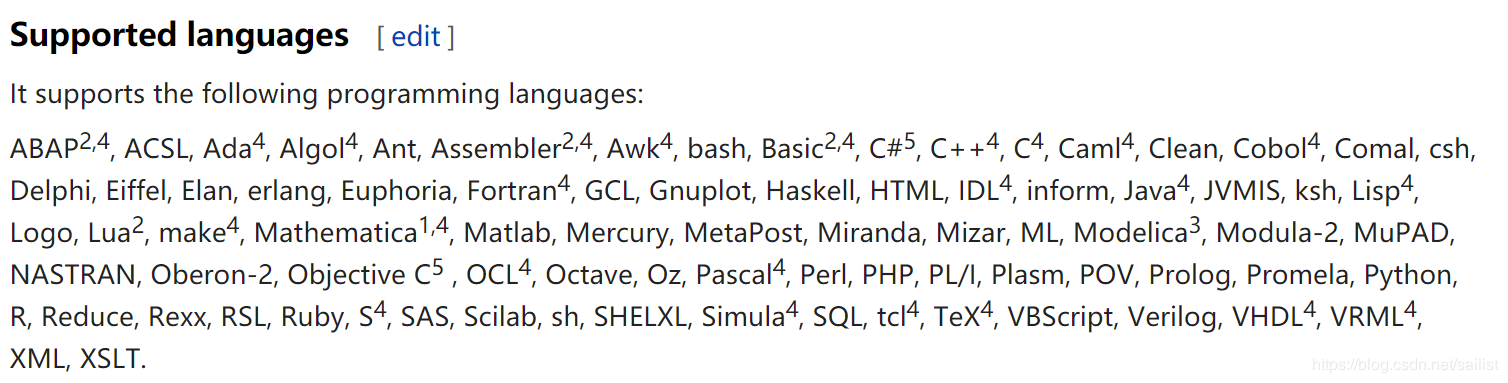
\includegraphics[width=0.8\textwidth]{C:/E/jupyter_notebook/marktex/output/images/53bb9cd2ced62c6673f39073ca9397b7.png}\vspace{\baselineskip}
\end{marktext}
\end{center}
\end{marktext}
\begin{lstlisting}[language={Python},keywordstyle=\color{blue!70},frame=shadowbox,showstringspaces=false,commentstyle=\color{red!50!green!50!blue!50},escapeinside=``,numbers=left,numberstyle=\small,basicstyle=\small]
if __name__ == "__main__":
	print("hello world!")
\end{lstlisting}


\begin{lstlisting}[language={C++},keywordstyle=\color{blue!70},frame=shadowbox,showstringspaces=false,commentstyle=\color{red!50!green!50!blue!50},escapeinside=``,numbers=left,numberstyle=\small,basicstyle=\small]
#include<stdio.h>
int main(){
	printf("hello world")
	return 0;
}

\end{lstlisting}
\begin{marktext}


\subsection{引用}


\end{marktext}
\begin{shaded}
\begin{marktext}
引用内环境和普通文本基本一致,但是不支持标题。
演示\textbf{加粗},\textit{斜体},\adjustbox{margin=1pt 1pt 1pt 2pt,bgcolor=aliceblue}{\small{行内代码}},$Inline Formula$,\href{http:///www.github.com}{超链接}
\end{marktext}


\begin{itemize}
\item
支持\textbf{加粗},\textit{斜体},\adjustbox{margin=1pt 1pt 1pt 2pt,bgcolor=aliceblue}{\small{行内代码}},$Inline Formula$,\href{http:///www.github.com}{超链接}
\end{itemize}


\begin{enumerate}
\item
支持\textbf{加粗},\textit{斜体},\adjustbox{margin=1pt 1pt 1pt 2pt,bgcolor=aliceblue}{\small{行内代码}},$Inline Formula$,\href{http:///www.github.com}{超链接}
\end{enumerate}






\end{shaded}


\begin{shaded}
\begin{marktext}
表格:
\end{marktext}


\begin{center}
\setlength\tablewidth{\dimexpr (\textwidth -4\tabcolsep)}
\arrayrulecolor{tablelinegray!75}
\rowcolors{2}{tablerowgray}{white}
\begin{tabular}{|p{0.500\tablewidth}<{\centering}|p{0.500\tablewidth}<{\centering}|}
\hline
\rowcolor{tabletopgray}
\textbf{ColA}&\textbf{ ColB }\\
\hline
 \textbf{Table Bold} &  \textit{Table Italic}\\
\hline
 \adjustbox{margin=1pt 1pt 1pt 2pt,bgcolor=aliceblue}{\small{Table Code}} &  $Table Formula$\\
\hline
\href{http:///www.github.com}{Table line}&Table Text\\
\hline
\end{tabular}
\end{center}


\begin{marktext}
公式:
\end{marktext}


\[
F(x_i) = wx_i+b\\
\]


\begin{marktext}
图片:
\begin{center}
\begin{marktext}
\vspace{\baselineskip}
\includegraphics[width=0.8\textwidth]{C:/E/jupyter_notebook/marktex/output/images/1c59f8ef2aa3c5e527a22b7c258489d6.png}\vspace{\baselineskip}
\end{marktext}
\end{center}


\end{marktext}


\end{shaded}


\end{document}